\documentclass[useAMS, usenatbib]{mnras}
\pdfsuppresswarningpagegroup=1
%
\usepackage[spanish,es-minimal,english]{babel}
\usepackage[utf8]{inputenc}
\usepackage{graphicx}
\graphicspath{{tere-figs/}{figs/}}

\usepackage{xcolor}
\usepackage{hyperref}
\usepackage{siunitx}
\usepackage{newtxtext}
\usepackage[stix2,smallerops]{newtxmath}
\usepackage{booktabs}
\hypersetup{colorlinks=True, linkcolor=blue!50!black, citecolor=black,
  urlcolor=blue!50!black}
\usepackage{etoolbox}
\robustify\bfseries
\robustify\itshape

\bibliographystyle{mnras}

\sisetup{
  % explicit""+" is useful for velocities
  retain-explicit-plus = true,
  % prefer 10^6 over 1 x 10^6
  retain-unity-mantissa = false,
  % Use x +/- e instead of x(e)  
  separate-uncertainty = true,
  % Make sure to pick up bold font when used in section heading for instance
  detect-weight = true,
}

%%
%% Will macros
%%
% A better \ion command that works in more circumstances
\newcommand\ION[2]{#1\,\scalebox{0.9}[0.8]{\uppercase{#2}}}
\newcounter{ionstage}
\renewcommand{\ion}[2]{\setcounter{ionstage}{#2}% 
  \ensuremath{\mathrm{#1\,\scriptstyle\Roman{ionstage}}}}
\newcommand\hii{\ion{H}{2}}
\newcommand\nii{[\ion{N}{2}]}
\newcommand\oiii{[\ion{O}{3}]}


%%
%% Teresa macros
%%
\newcommand{\Sub}[1]{_\mathrm{#1}}
\newcommand{\SSub}[1]{_\mathrm{\scriptscriptstyle #1}}
\newcommand{\Sup}[1]{^\mathrm{#1}}
\newcommand{\kms}{\ensuremath{\mathrm{km\ s}^{-1}}}
\newcommand{\pcc}{\ensuremath{\mathrm{cm}^{-3}}}
\newcommand{\sii}{[\ion{S}{2}]}
\newcommand{\heii}{\ion{He}{2}}
\newcommand\OIlam{[\ion{O}{1}]\,6300\,\AA\@}
\newcommand\SIIlam{[\ion{S}{2}]\,6731\,\AA\@}
\newcommand\SIIlamshort{[\ion{S}{2}]\,6716\,\AA\@}
\newcommand\SIIlamboth{[\ion{S}{2}]\,6716,6731\,\AA\@}
\newcommand\SIIIlam{[\ion{S}{3}]\,6312\,\AA\@}
\newcommand\NIIlam{[\ion{N}{2}]\,6584\,}
\newcommand\NIIlamlam{[\ion{N}{2}]\,6548,6584\,\AA\@}
\newcommand\OIIIlam{[\ion{O}{3}]\,5007\,\AA\@}
\newcommand\HeIIlam{HeII\,4686\,\AA\@}
\newcommand\Halam{H$\alpha$\,6563\,\AA\@}
\newcommand\Ha{\ensuremath{\mathrm{H}\alpha}}
\newcommand\Hb{\ensuremath{\mathrm{H}\beta}}
\newcommand{\vhel}{\ensuremath{V_\mathrm{hel}}}
\newcommand{\vmean}{\ensuremath{\langle V\rangle}}
\newcommand{\vsys}{\ensuremath{V_\mathrm{sys}}}
\newcommand{\vexp}{\ensuremath{V_\mathrm{exp}}}
\newcommand{\hr}{\ensuremath{^\mathrm{h}}}
\newcommand{\minute}{\ensuremath{^\mathrm{m}}}
\newcommand{\teff}{\ensuremath{T_\mathrm{eff}}}


\title{The complex structure and peculiar internal motions of the planetary nebula NGC 6210}

%\author{Ma.\ T. Garc\'{\i}a-D\'{\i}az, J. A. L\'opez, W. Steffen \& 
%  M. G., Richer 
% \affil{Instituto de Astronom\'ia,
%    Universidad Nacional Aut\'onoma de M\'exico} Campus Ensenada,
%  Ensenada, Baja California, 22800, M\'exico}
%\affil{tere@astrosen.unam.mx, jal@astrosen.unam.mx, wsteffen@astrosen.unam.mx, richer@astrosen.unam.mx}

\author[López et al.]{
  J. A. López,\(^1\)\thanks{
    jal@astro.unam.mx,
    tere@astro.unam.mx,
    w.henney@irya.unam.mx,
    richer@astro.unam.mx
  }
  Ma.\ T. García-Díaz,\(^1\)\footnotemark[1]
  William J. Henney\(^2\)\footnotemark[1]
  and M. G. Richer\(^1\)\footnotemark[1]
  \\
  \(^1\)\foreignlanguage{spanish}{
    Instituto de Astronomía,
    Universidad Nacional Autónoma de México,
    Ensenada, Baja California, 22800, México}
  \\
  \(^2\)\foreignlanguage{spanish}{
    Instituto de Radioastronomía y
    Astrofísica, Universidad Nacional Autónoma de México, Apartado
    Postal 3-72, 58090 Morelia, Michaoacán, Mexico}
}
% These dates will be filled out by the publisher
\date{Accepted XXX. Received YYY; in original form ZZZ}

% Enter the current year, for the copyright statements etc.
\pubyear{2020}




\begin{document} 
\label{firstpage}
\pagerange{\pageref{firstpage}--\pageref{lastpage}}
\maketitle

\begin{abstract}
  A comprehensive kinematic study has been carried out on the planetary nebula (PN) NGC 6210. Multiple long-slits, echelle spectra have been obtained over the face of this nebula mapping its full shell structure, the opposite pairs of extended, twisted arms and the bipolar collimated outflows and bullets. Public {\it HST} imagery has been used to identify kinematic elements with structural components. The long-slit spectroscopic information has been combined into channel maps that greatly facilitate visualizing the otherwise intricate expansion pattern of this  planetary nebula. The global morphology of NGC 6210 is  reminiscent of other planetary nebulae with extended X-ray emission, suggesting the presence of a central hot bubble produced by shocked stellar wind. In spite of the dramatic structure of this PN substantial expanding radial motions are only found in the material surrounding the central, inner shell. The slow radial motions of the collimated outflows and the bullet-like knots indicate that they are  moving away from the core very close to the plane of the sky, nearly perpendicular to the line of sight
\end{abstract}


\begin{keywords}
  Planetary Nebulae: individual (NGC~6210)
  -- ISM: kinematics and dynamics -- ISM blowout
  -- techniques: imaging spectroscopy
\end{keywords}

\maketitle

\section{INTRODUCTION}
\label{sec:introduction}
NGC 6210 is a bright and relatively large PN in the northern sky. The first photographic image of NGC 6210 was published by \citet{Duncan:1937a}. In that old, fuzzy image a pair of twisted arms protruding in opposite directions from a blurred,  bright, nebular core are apparent. Several studies have discussed the inner kinematic motions of this object, e.g. \citet{Osterbrock:1966a, Weedman:1968a, Becker:1984a, Icke:1989a}. However, none of those studies had the spatial coverage and spectral resolution needed to produce a reliable spatio-kinematic model of this PN. 
The best kinematic study to date on NGC 6210 is probably the one published by \citet{Phillips:1996a}  who obtained 11 long-slits centered on the nebular core, with each slit at different position angles thus providing a good spatial coverage but with only limited, low and medium spectral resolution. From these data  they suggested a  reasonable kinematic model for the ionized nebula. NGC 6210 jumped into fame thanks to the {\it HST} images obtained during the 1996 - 1998 period under the observing programs 6347 (K. Borkowski), 6792 (R. Rubin), 7501 (A. Hajian)  and 11122 (B. Balick). These images showed for the first time the extraordinarily complex morphology of NGC 6210. Incidentally the  {\it HST} and ground-based imagery prompted the nickname "the turttle" for this nebula, given the shape of its main body and extended arms that resemble the shell of a turttle with a long neck and its fins. The distance estimates to NGC 6210 vary roughly from 1.5 to 2.0 kpc. \citep{Hajian:1995a} derive a distance to NGC 6210 from VLA 6 cm  expansion parallax measurements of 1.57$\pm0.40$ kpc, considering an expansion distance of 23 \kms 

In this work we present a thorough spectral mapping of all the morphological elements of the PN obtained at high spectral resolution that allow 
disentangling the various spatio-kinematic components and provide and overall view of its structure and evolution. Radial velocities are combined with 2-epoch HST \oiii and \nii archive image sets (http://archive.stsci.edu/) to derive proper motions. Individual long-slit echelle data obtained over N observing runs are combined into emission and velocity channel maps that serve as an excellent tool to visualize and understand the peculiar velocity fields, of the several structural components.

In Section 2, we describe our observations and the data-reduction steps, In Section 3 we describe the velocity-channel map of emission. In Section 4, we discuss the radial velocities and proper motions of the nebula. In Seccion 5 we present the discussion and conclusion.

\section{OBSERVATIONS AND DATA REDUCTION}
\label{sec:observations}

Long-slit, echelle, spectroscopic observations of the nebula NGC~6210
were performed with the 2.1~m telescope at the Observatorio
Astron\'omico Nacional at San Pedro M\'artir, (OAN-SPM), Baja
California, M\'exico. We used the Manchester Echelle Spectrometer
(MES-SPM) \citep{Meaburn:2003a} on the 2.1 m telescope in its $f$/7.5
configuration.  The MES-SPM is a long-slit, echelle spectrometer that
has no cross-disperser; it isolates single orders using interference
filters. For the 2003, 2004 and 2011 of the present observations, we used a
SITE-3 CCD detector with 1024 $\times$ 1024 square pixels, each 24
$\mu$m on a side ($\equiv$0.312 arcsec pixel$^{-1}$). The detector
was set to a binning of 2 $\times$ 2 in both the spatial and spectral
directions. Consequently, 512 increments, each 0\farcs624{} long gave
a projected slit length of 5\farcm32 on the sky. A TEK-1 CCD detector
was used for the 1998 data set with 1024$\times$1024 pixels$^2$ with
sides measuring 24 $\mu$m, using 2$\times$2 binning ($\equiv$0.62 arcsec
pixel$^{-1}$ and 3.5 \kms pixel$^{-1}$). For the 2001 and 2013 we used
a Marconi CCD detector with 2048 $\times$ 2048 square pixels, each 13.6
$\mu$m on a side. The detector was set to a binning of 2 $\times$ 2 in
both the spatial and spectra directions. Consequently, 1024
increments, each 0\farcs352{} long gave a projected slit length of
5\farcm47 on the sky.

We used a 90\,\AA\, and 50\,\AA\, bandwidth
filter to isolate the 87th and 114th orders containing the
\Ha\,$+$\,\NIIlam\, and \OIIIlam\, nebular emission lines,
respectively. We used a 70~$\mu$m{} ($\equiv$0.95\arcsec) slit, giving
a velocity resolution of 9.2 \kms{} ($\equiv$0.312 arcsec
pixel$^{-1}$ and 150 $\mu$m{} ($\equiv$1\farcs 9 and $\equiv$11.5
\kms) slit.


We obtained 23 consecutive and tightly spaced positions over the
NGC~6210. The slit positions are indicated and labeled in Figure~1 on
a WFPC~2 image of the NGC~6210 obtained from the HST archive. In order
to establish the exact position of the slit in each pointing, the slit
position on the sky was recorded with an automatic procedure available
in MES-SPM prior to the spectroscopic exposure.

The log of spectroscopy observation is given in Table 1 divided into
dates, number of spectra, exposure times, spectral range, resolution,
slit wide, position angle and name of the slit (see Figure~1). 
The high resolution data are available in San Pedro M\'artir Kinematic Catalogue
of Galactic Planetary Nebulae (http://kincatpn.astrosen.unam.mx)
\citep{Lopez:2012a}.


Due to saturation of several slit positions on the nebula, we obtained a 
new set of observation on August 13, 2015. We used the same detector as 
that used for the 2015 dataset, which was a E2V-4240 (Marconi 2)  detector 
with 2048$\times$2048 pixels$^2$ 
with sides measuring 13.5 $\mu$m, using 2$\times$2 binning 
($\equiv$0.531 arcsec pixel$^{-1}$. Spectra were obtained at 11 different 
positions across the nebula, with exposure times of 1800 seconds. The slit 
was oriented N-S. 

An additional slit was placed outside the nebula 
to detect The outer halo of NGC 6210. The observation was carried out on 18 September 2019.  The spectrum was obtained in order 87 (H alpha and [N II] lines) with the 150 micron slit oriented at position angle of 56 degrees.  The detector was an E2V 2048x2048 CCD with 13.5 $\mu$/pix used in binning 3$\times$3.  The spectral dispersion was 0.084 \AA/pix and the plate scale 0.175\arcsec/pixel.

The characteristics of the observations are listed in Table 2.

\begin{table*}
\centering
\caption{Log  of Time-resolved  Observations of {\bf NGC~6210}.}
\begin{tabular}{l|ccccccc} \hline 
&  \multicolumn{7}{c}{Spectroscopy hight resolution/ 2.1m  OAN-SPM}            \\[0.1pt]
\hline 
Run    &   Exp. Time & Range  & slit & P. A.   & slit        \\
DD/MM/YYYY   &     frame         &    (s)   &  (\AA)    &    (\AA)  & (m$\mu$) & (degree) & name    \\[1pt]   \hline 
28/06/1998          & 30 & H$\alpha$  & 150 & 90 & o\\
28/06/1998          & 300 & H$\alpha$  & 150 & 90 & n\\
28/06/1998           & 1200 & H$\alpha$   & 150 & 90 & m,p,q \\
05/06/2003         & 1800 &  H$\alpha$   & 70 &0 & f,e,d,h,i,k,b\\ 
16/10/2003   &  1800 &   H$\alpha$    & 70 & $-$21 & t\\
16/10/2003    &  1800 &   H$\alpha$   & 70 & $-$68 & v\\
17/10/2003    &  1800 &   H$\alpha$  & 70 & 77 & w\\
13/06/2004   & 1800 &   O\sc{iii}  & 70 & $-$9 & r  \\  
13/06/2004   & 1800 &   O\sc{iii}  & 70 & $-$19 & s  \\  
14/06/2004    & 1800 &   S\sc{ii} &150 & $-$19 & s  \\
13/06/2004   & 1800 &   O\sc{iii}  & 70 & $-$56 & u  \\  
14/06/2004   & 1800 &   O\sc{iii}  & 150 & 0 & a,l  \\
21/05/2011     & 1800 & H$\alpha$  & 150 & 0 & g \\
21/05/2011     & 600 & O\sc{iii} & 150 & 0  & g\\
06/07/2013    &  1800 & H$\alpha$   & 150 & 0 & c,i,j \\
20/08/2005   & 3 &  1800 &   H$\alpha$, [OIII]    & 0.26 & 70 & 0 & h, j, k\\
\hline
\hline 
\end{tabular}
\label{table:pa5}
\end{table*}


\begin{table*}
\centering
\caption{Log  of Time-resolved  Observations of {\bf NGC~6210}. Epoch 2015}
\begin{tabular}{l|ccccccc} \hline 
&  \multicolumn{7}{c}{Spectroscopy hight resolution/ 2.1m  OAN-SPM}            \\[0.1pt]
\hline 
Run   &   Exp. Time & Range  & slit & P. A.   & slit        \\
DD/MM/YYYY   &     frame         &    (s)   &  (\AA)    &    (\AA)  & (m$\mu$) & (degree) & name    \\[1pt]   \hline 
18/08/2015  &  1800 &   H$\alpha$, [OIII]  & 70 & 0 & c, d, e, f, g\\
19/08/2015  &  1800 &   H$\alpha$, [OIII]   & 70 & 0 & b, a, i\\
19/08/2015  &  1800 &   H$\alpha$    & 70 & 0 & b, a, i\\
18/09/2019  &  1800 &   H$\alpha$    & 150 & 56 & \\

\hline
\hline 
\end{tabular}
\label{table:pa5}
\end{table*}

All data was reduced (bias removal 
and cosmic-ray removal) by using standard IRAF\footnote{IRAF is
  distributed by the National Optical Astronomy Observatory, which is
  operated by the Association of Universities for Research in
  Astronomy, Inc. under cooperative agreement with the National
  Science foundation}.
  This was followed by rectification and first-order wavelength 
  calibration of the two-dimensional spectra based on the comparison
  the spectrum
of a Th/Ar lamp to an accuracy of $\pm$1 \kms{} when converted to
radial velocity.  All spectra presented in this paper are corrected to
heliocentric velocity (\vhel). 
The Figure 3 shows the position-velocity ({\it P-V})  arrays of \Halam\,
\NIIlam \AA, \OIIIlam, respectively, where the heliocentric velocities are used,
and positions are specified as arcsecond offsets (x,y).

Using FORTRAN and phython routines, we produced  velocity cubes in  \NIIlam{} and \oiii{} emission lines, in order to 
...

The resulting data cubes for the \Halam\, and \NIIlam\, lines are shown
in Figure 3 as isovelocity channel maps, each isovelocity map is 20
\kms\, wide. 


\section{KINEMATICS}
\label{sec:kinematic}

The Figure 3 shows the \Halam{},  \OIIIlam{}, and \NIIlam{} velocity arrays, {\it P--V}, for all individual slit position, observed on 2015 epoch: \Ha{} {\it P--V} is shown on the left panel,  on
the middle panel is the corresponding \OIIIlam\, {\it P--V} and \NIIlam{} on the right panel. Spatial
offsets are in arcseconds.  The stellar continuum from the central star
has not been subtracted. We derive a heliocentric
systemic velocity, \vsys $=40$~\kms{} by using the slits position f (epoch 2003) and  which passes through the central star. The expansion velocity of the inner shell, v$_{exp}$ = 28 \kms.





 % \caption{{\it Left:} Location of each slit position is indicated and
 %   labeled on an HST \OIIIlam, image of the NGC~6210. North is up,
 %   east left}

\begin{figure*}
\centering
  \includegraphics[width=0.7\textwidth]{Figure1.pdf}
  \caption{ }
\end{figure*}

\begin{figure*}
\centering
  \includegraphics[width=0.4\textwidth]{Figure2a.pdf}
  \caption{ }
\end{figure*}


\begin{figure*}
\centering
  \includegraphics[width=1\textwidth]{Figure3.pdf}
  \caption{ }
\end{figure*}









\begin{figure*}
\centering
\includegraphics[width=0.9\textwidth]{Figure8.png}
\includegraphics[width=0.42\textwidth]{N6210_ruso.pdf}
\quad
\includegraphics[width=0.427\textwidth]{opo9836f.jpg}
  \caption{}
\end{figure*}





\begin{figure*}
\centering
\includegraphics[width=0.9\textwidth]{Figure6.pdf}
  \caption{  }
\end{figure*}





\begin{figure*}
\centering
\includegraphics[width=0.9\textwidth]{rendija-c-cont.pdf}
  \caption{  }
\end{figure*}



\begin{figure*}
\centering

\includegraphics[width=0.4\textwidth]{slit_t_ha_nii.pdf}
\includegraphics[width=0.4\textwidth]{slit_v_ha_nii.pdf}
\includegraphics[width=0.4\textwidth]{slit_w_ha_nii.pdf}
\includegraphics[width=0.2\textwidth]{slit_u_oiii.pdf}
\includegraphics[width=0.2\textwidth]{slit_s_oiii.pdf}
\includegraphics[width=0.2\textwidth]{slit_r_oiii.pdf}

  \caption{  }
\end{figure*}



\clearpage

\begin{figure}
  \centering
  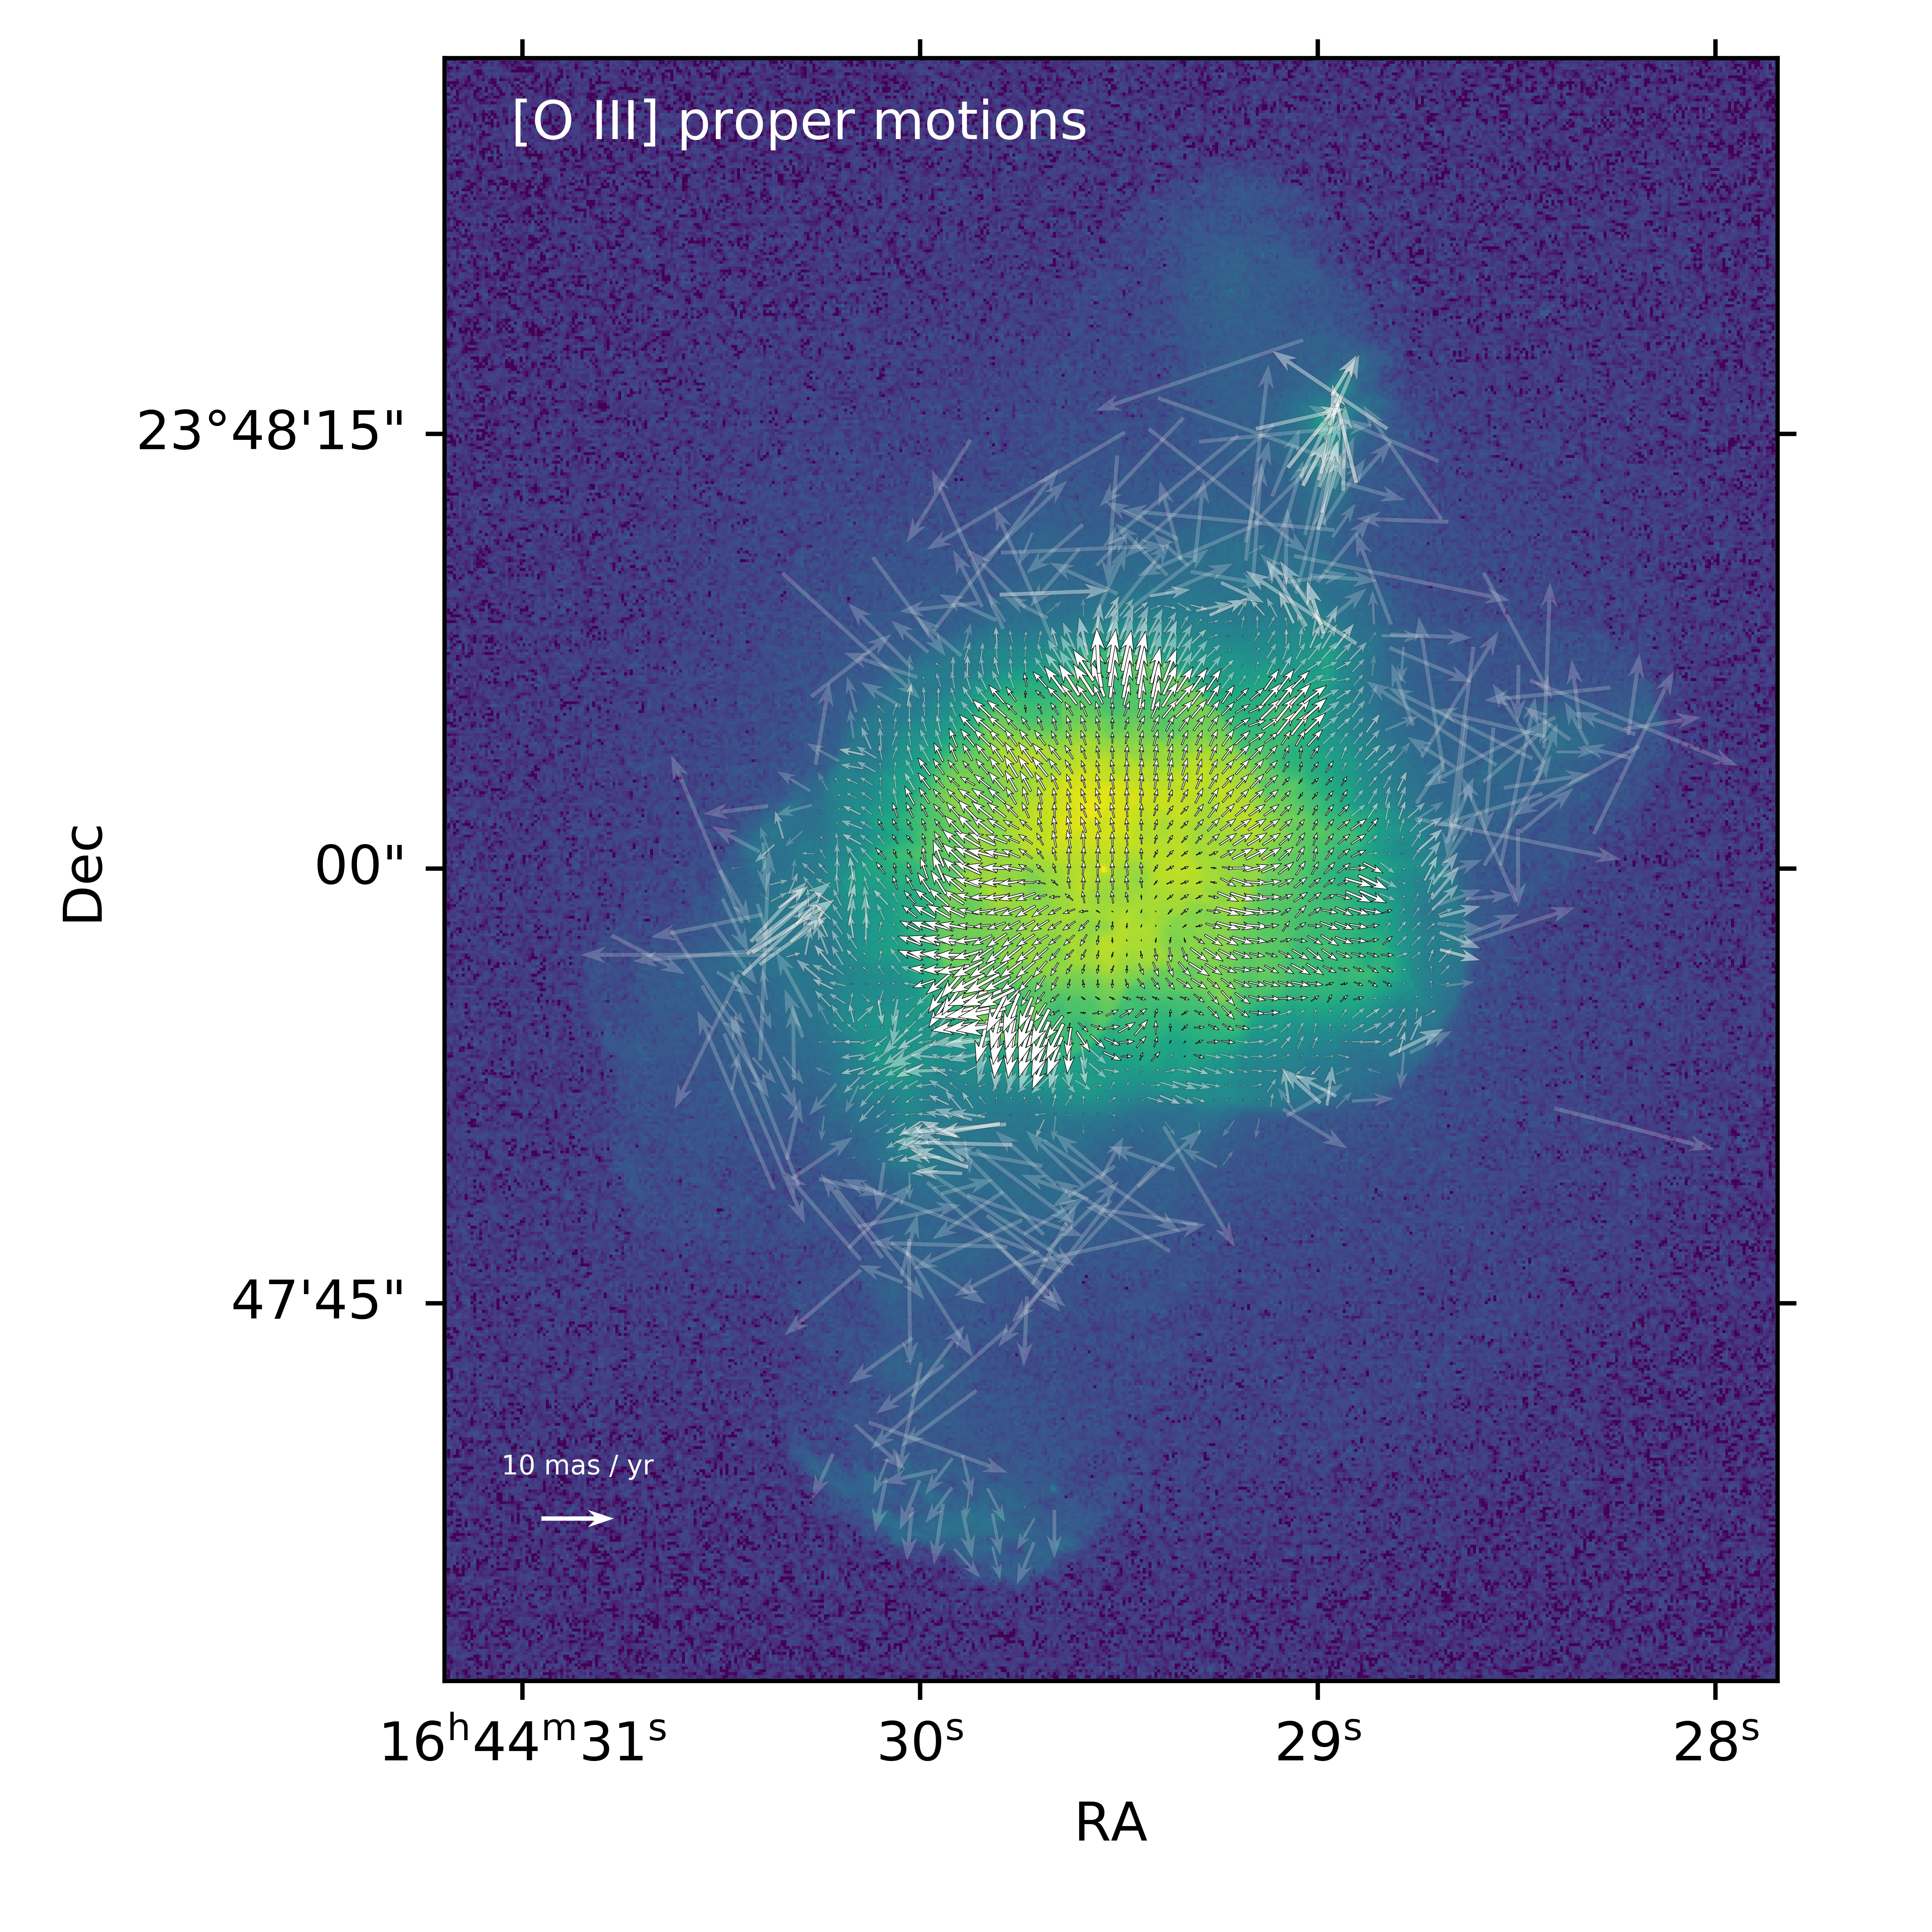
\includegraphics[width=\linewidth]{oiii-propermotions}
  \caption{Proper motions derived from two HST \oiii{} images (F502N
    filter) separated by 10.45 years, using the FLCT algorithm with a
    Gaussian window width of 10~pixels. The key at bottom left shows a
    proper motion of \SI{10}{mas.yr^{-1}}, corresponding to
    \SI{95}{km.s^{-1}} for an assumed distance of \SI{2}{kpc}.}
  \label{fig:proper-motions-oiii}
\end{figure}
\begin{figure}
  \centering
  \includegraphics[width=\linewidth]{nii-propermotions}
  \caption{As Fig.~\ref{fig:proper-motions-oiii} but for two HST
    \nii{} images (F658N filter). Note that the field of view is
    cropped slightly smaller than for \oiii{}.}
  \label{fig:proper-motions-nii}
\end{figure}

\begin{figure*}
  \centering
  \includegraphics[width=\linewidth]{turtle-peanut-map}
  \caption{
    Velocity features in the high-ionization shells,
    which have been identified in the \oiii{} slits.
    Left panel shows blue-shifted features,
    while right panel shows red-shifted features,
    each labelled with their line-of-sight velocity
    with respect to the nominal systemic velocity of \SI{40}{km.s^{-1}}.
    Solid lines show features in the inner shells,
    dashed lines show features in the intermediate shell,
    and dot-dashed lines show miscellaneous features between the two shells.
    The line width is a qualitative indicator of the brightness of each feature.
  }
  \label{fig:shell-velocity-components}
\end{figure*}

\begin{figure}
  \centering
  \includegraphics[width=\linewidth]{turtle-shell-velocity-axes-annotated}
  \caption{
    Radial velocity versus position
    for the shell features shown in Fig.~\ref{fig:shell-velocity-components}.
    Results are shown along two axes:
    Axis~A (upper panel) is the apparent major projected axis of the inner shells,
    while Axis~B (lower panel) is perpendicular to this.
    Large blue circles show the inner shell,
    small red circles show the intermediate shell,
    and green triangles show miscellaneous features between the two shells.
    Darker colors indicate features that are closer to each respective axis.
    Colored lines are merely to guide the eye,
    and show possible interpretations of the shell kinematics along the two axes.
  }
  \label{fig:shell-velocity-axes}
\end{figure}


\newpage
\section{Proper motions}
\label{sec:proper-motions}

The data used in this study to measure the proper motions of the turttle nebula consist of images which were retrieved from the HST archive. The \nii{} observations were made in two separate observing runs: on 1998 June 30, as part of program 7501, with Hajian, Arsen R., as PI. During this run, six images were obtained with the WFPC2, with an exposure time of 100 s (three images) y 40 s (three images) using the F658N filter. The second-epoch data were obtained on 2008 January 18, from the science program 11122, with Bruce Balick, as PI, who employed the same configuration as in program 7501 to acquire three images with the F658N filter, using 400 s exposure times for all of them. For all of the images, we used the drizzled images (processed with Astrodrizzle). 

Proper motions are calculated from HST WFPC2 imaging at two epochs separated by approximately 10 years,
using the FLCT method \citep{Welsch:2004a, Fisher:2008a}.\footnote{
  We used version 1.07 of FLCT, obtained from \url{http://cgem.ssl.berkeley.edu/cgi-bin/cgem/FLCT/home},
  together with version 1.04 of the Python wrapper pyflct,
  obtained from \url{https://github.com/PyDL/pyflct}.}
Results are shown in Figures~\ref{fig:proper-motions-oiii} and~\ref{fig:proper-motions-nii} for \oiii{} and \nii{}, respectively.
In both cases, the images were remapped to a uniform square pixel grid at the WFC resolution of \SI{0.1}{arcsec.pix^{-1}} before applying the algorithm.
The resultant per-pixel motions between the two epochs are found to be of order \SI{0.5}{pix} (\(\approx \SI{5}{mas.yr^{-1}}\))
and these raw results were then corrected by applying a global shift to force the motion of the central star to be zero.
The systematic error from the global alignment of the two epochs is estimated to be \SI{1.5}{mas.yr^{-1}},
which is expected to dominate the proper motion uncertainties in the brighter parts of the nebula.
In fainter and more featureless regions of the nebula, the proper motions are increasingly affected by random noise,
which can be seen in parts of the lobes in Figure~\ref{fig:proper-motions-oiii}.

The corrected results, as shown in the figures, can be seen to display motions that are predominantly radial from the central star.
To convert the angular motions into transverse velocities, we assume a distance of \SI{2}{kpc},
so that \SI{10}{mas.yr^{-1}} is equivalent to \SI{95}{km.s^{-1}}.
From the \oiii{} images (Fig.~\ref{fig:proper-motions-oiii}),
the fastest plane-of-sky motions are of order \SI{60}{km.s^{-1}},
and are chiefly along the NNW--SSE direction,
including the projected major axis of the inner peanut shell,
the NW~knot, the N~jet, and the end-cap of the S~lobe.
Motions along the perpendicular ENE--WSW direction are typically slower,
of order \SI{30}{km.s^{-1}}.
Note that proper motions are unavailable for the end cap of the N lobe since the second epoch HST image does not cover this region.

The \nii{} images (Fig.~\ref{fig:proper-motions-nii}) show a similar expansion pattern for the features that are visible in both lines.
Remarkably low plane-of-sky velocities of \(\le \SI{15}{km.s^{-1}}\) are seen for the \nii{}-bright knot complexes immediately north and west of the central star. 

\section{Kinematic components from slit spectra}
\label{sec:kinematic-components}

In order to investigate the kinematics of the nebula in detail,
we have measured the velocities of distinct emission components in each slit spectrum
and organized them into broad systems based on their location, morphology and degree of ionization.

\subsection{High-ionization shells}
\label{sec:high-ioniz-shells}

These systems represent the majority of the \oiii{} emission in the core of the nebula
and show a nested elliptical shell morphology.
Figure~\ref{fig:shell-velocity-components} shows the \oiii{} emission components associated with these shells,
as derived from the longslit spectra.
Line-of-sight velocities are given with respect to the nominal systemic velocity (\SI{40}{km.s^{-1}} heliocentric),
separated into negative velocities (left panel) and positive velocities (right panel).
The inner ``peanut'' shells, with a radius of \(5''\) to \(7''\), are the brightest
and are indicated by thick-lined colored ellipses. 
The edge of the more extended intermediate shell, with a radius of \(8''\) to \(12''\), is 10 to 100 times fainter than the inner shells
and is indicated by thinner dashed ellipses.
Additional miscellaneous emission features located in between these shells are indicated by dot-dashed ellipses.
Further features that seem to be associated with the low-ionization knots discussed below in \S~\ref{sec:knot-complexes} are omitted from the figure.


Although the inner shell is irregular in shape,
it shows an apparent elongation along \(\text{PA} \approx \ang{160}\).
The intermediate shell is elongated roughly perpendicular to this, along \(\text{PA} \approx \ang{70}\).
In Figure~\ref{fig:shell-velocity-axes} we plot the velocity of each shell component
against position along each of these axes,
which we denote axis~A and axis~B.  
Each component was assigned to only one axis (A or B), according to its location,
but this assignment is unavoidably subjective for components near the center,
where the two axes cross.

Along axis~A a closed velocity ellipse can be seen for the inner shells,
with a maximum splitting of \(\pm \SI{22}{km.s^{-1}}\) close to the central star
and velocities close to zero at either end (\(\pm 7''\)).
The pattern is not entirely symmetric,
with a slight gradient of \(\pm \SI{3}{km.s^{-1}}\) along the length,
in which the more negative velocities are at the SSE end.
The centroid of the ellipse is also shifted by \(\SI{-3.5}{km.s^{-1}}\)
with respect to the systemic velocity.

Along axis~B,
which is the apparent minor axis of the inner shells (\(\pm 5''\)),
the ellipse is distorted and the gradient is much more pronounced:
\(\pm \SI{11}{km.s^{-1}}\),
with the more negative velocities at the ENE end
(large blue circle symbols in lower panel of Fig.~\ref{fig:shell-velocity-axes}).
Velocity splitting of \(\pm \SI{9}{km.s^{-1}}\) is seen near both ends,
but it is not clear from the \oiii{} spectra if the ends are closed or open,
since none of the \oiii{} slits are aligned with this axis.
However, one of the \nii{} slits (slit~W) is indeed oriented close to axis~B and,
although the shells emit only weakly in \nii{},
the distorted ellipse is clearly closed at the ENE end
(large pink triangle symbol in Fig.~\ref{fig:shell-velocity-axes}).
The situation is not so clear at the WSW end
since any \nii{} emission from the shell is swamped by brighter emission from the knot complexes.
However, the evidence from \textit{HST} imaging suggests that the shell is closed in this direction also.

The intermediate shell along axis~B repeats a similar kinematic pattern to the inner shell,
but at larger radii.
It is represented by dashed ellipses in Figure~\ref{fig:shell-velocity-components} and small red circle symbols in Figure~\ref{fig:shell-velocity-axes}.
The gradient (\(\pm \SI{9}{km.s^{-1}}\)) and splitting (\(\pm \SI{8}{km.s^{-1}}\))
are both marginally smaller than for the inner shell.
Note that, unlike the inner shells, the intermediate shell is markedly lop-sided,
extending \(12''\) to the WSW, but only \(10''\) to the ENE.

The miscellaneous high-ionization components lie outside the inner shells
and show a spoke-like morphology on the \textit{HST} images.
It is represented by dot-dashed ellipses in Figure~\ref{fig:shell-velocity-components} and small green triangle symbols in Figure~\ref{fig:shell-velocity-axes}.
They do not show any marked kinematic pattern,
but are broadly compatible with the velocities of nearby portions of the intermediate shell. 

\subsection{Low-ionization knot complexes}
\label{sec:knot-complexes}

\begin{figure*}
  \centering
  \includegraphics[width=\linewidth]{turtle-knot-complex-map}
  \caption{
    Velocity features in the low-ionization knot complexes,
    which have been identified in the \nii{} slits.
    Left panel shows blue-shifted features,
    while right panel shows red-shifted features,
    each labelled with their line-of-sight velocity
    with respect to the nominal systemic velocity of \SI{40}{km.s^{-1}}.
    The line width is a qualitative indicator of the brightness of each feature.
  }
  \label{fig:knot-complex-map}
\end{figure*}

\begin{figure*}
  \centering
  \includegraphics[width=\linewidth]{turtle-nii-knot-complexes}
  \caption{
    Reconstructed velocity channel maps from the \nii{} slit spectra,
    showing the red-shifted (left panel) and blue-shifted (right panel) knot complexes.
    Note that channel maps have not been spatially interpolated,
    so that the individual slit positions can be seen.
    Each color image is constructed from 3 channels, each of width \SI{20}{km.s^{-1}},
    as indicated on the figure.
    All velocities are with respect to the nominal heliocentric systemic velocity of \SI{-40}{km.s^{-1}}.
    The low-ionization emission components from Fig.~\ref{fig:knot-complex-map}
    have been classified into 5 knot complexes,
    which are shown as colored outlines. 
  }
  \label{fig:knot-complexes}
\end{figure*}

\begin{figure}
  \centering
  \includegraphics[width=\linewidth]{turtle-knot-complexes-velocity-axes-annotated}
  \caption{
    Radial velocity versus position
    for the low-ionization features features shown in Fig.~\ref{fig:knot-complex-map}.
    Results are shown projected along along the same two axes,
    Axis~A (upper panel) and Axis~B (lower panel),
    as in Fig.~\ref{fig:shell-velocity-axes},
    but this time each feature is shown projected along both axes.
    The features are divided into different knot complexes,
    as shown in Fig.~\ref{fig:knot-complexes},
    which are indicated by symbol type and color.
    Symbol size is proportional to feature brightness (log scale)
    and symbol shade indicates position along the other axis (darker is more positive).
    Continuous lines show the same high ionization shells
    as in Fig.~\ref{fig:shell-velocity-axes}.
  }
  \label{fig:knot-complex-velocity-axes}
\end{figure}

The \nii{} emission from the nebula is dominated by small-scale knots,
as can be appreciated on the \textit{HST} images (Figure~XXX).
These knots have typical sizes \(< 1''\) and so are not spatially resolved
in our ground-based spectroscopy.
A small number of isolated knots are individually detected in our spectra,
but in general we detect only the combined emission of extended knot complexes.
Figure~\ref{fig:knot-complex-map} shows all the \nii{} emission components
identified from our spectra, but excluding those associated with the high-ionization
shells discussed above.
As previously, the components are divided into negative (left panel)
and positive (right panel) velocities.  
In Figure~\ref{fig:knot-complex-velocity-axes}
we classify the emission components into five knot complexes,
plus three individual knots, whose plane-of-sky distribution
and typical line-of-sight velocity are shown
superimposed on the \textit{HST} \nii{} image (contours)
and isovelocity channel maps reconstructed from our slit spectra (color images).

Figure~\ref{fig:knot-complexes} shows the velocity of each \nii{} component
as a function of position along the two axes that characterize the high-ionization shells:
axis~A at \(\text{PA} = \ang{160}\)
and axis~B at \(\text{PA} = \ang{70}\) (see \S~\ref{sec:high-ioniz-shells}).
The kinematics of the shells themselves are shown by faint continuous lines for comparison.
Note that the extent of the velocity axis in this figure
is twice as large as in Figure~\ref{fig:shell-velocity-axes}. 

The clearest axial alignment is seen for the SW Red complex,
which is very tightly clustered around the negative arm of axis~B.
The same is seen to a lesser extent for the NE Blue complex
around the positive arm of axis~B,
but the distribution around the axis is broader in this case.
The remaining complexes have no clear alignment with either axis,
except that the SE Blue complex is marginally more elongated
along the positive arm of axis~A.

The upper panel of Figure~\ref{fig:knot-complex-velocity-axes} indicates
that there is no clear velocity gradient along axis~A,
but the low-ionization knots have significantly faster radial velocities
than the high-ionization shells, by roughly a factor of two.
In addition, there is an asymmetry between the blue and red components:
the blue-shifted knot complexes tend to have a larger radial velocity magnitude,
but to have fainter \nii{} emission, as compared with the red-shifted knot complexes.

From the lower panel of Figure~\ref{fig:knot-complex-velocity-axes},
it is apparent that there is a significant gradient of \(\approx \SI{20}{km.s^{-1}}\)
along axis~B, which is seen in both blue-shifted and red-shifted components.
The sense of this gradient is the same as that seen in the high-ionization shells
along this axis.
It is mainly due to velocity differences
\emph{between} complexes rather than within them,
although both the SW Red and NE Blue complexes
show significant internal gradients of \(\approx \SI{10}{km.s^{-1}}\) in the same direction.

There is an approximate kinematic and spatial symmetry
between pairs of opposite knot complexes:
SW Red with NE Blue complex, and N Red with SE Blue.
It is possible that the west and east sides of the N Red complex
are actually two separate complexes,
in which case the east side would pair with the SW Faint Blue complex,
which would further reinforce this symmetry.

\subsection{Outer lobes}
\label{sec:outer-lobes}

\begin{figure*}
  \centering
  \includegraphics[width=\linewidth]{turtle-lobes-simplified}
  \caption{
    Velocity components and systems in the outer lobes.
    (a)~Blue-shifted components identified in individual slits.
    (b)~Red-shifted components identified in individual slits.
    (c)~Classification of components into seven high-velocity systems (colored shapes)
    along three different axes (heavy dashed lines).
    (d)~Same but for eleven intermediate velocity systems.
  }
  \label{fig:outer-lobe-components}
\end{figure*}
\newcounter{Syscounter}
\newcommand\Sys[1]{%
  \setcounter{Syscounter}{#1}%
  \ensuremath{\mathrm{\Roman{Syscounter}}}%
}
\newcommand\SysP[1]{\ensuremath{\Sys{#1}^+}}
\newcommand\SysM[1]{\ensuremath{\Sys{#1}^-}}

The emission from the outer lobes is much fainter than the inner shells,
and is most easily detected in \oiii{}.
Figure~\ref{fig:outer-lobe-components} shows all the outer lobe velocity components
that we have been able to measure from the \oiii{} slits:
blue-shifted components in panel~a and red-shifted components in panel~b.
As with the low-ionization knot complexes (see \S~\ref{sec:knot-complexes}),
there are many apparent pairings between blue and red components on opposite sides of the nebula.
This is illustrated in the lower panels of Figure~\ref{fig:outer-lobe-components},
where we classify the components into four high-velocity systems,
\Sys{1} to \Sys{4}
with \(|V| = \text{\SIrange{18}{25}{km.s^{-1}}}\) (panel~c)
and six intermediate-velocity systems,
\Sys{5} to \Sys{10}
with \(|V| = \text{\SIrange{5}{14}{km.s^{-1}}}\) (panel~d).
Nearly all of these systems have a blue and a red component
which are approximately symmetrically arranged about the central star.
For instance, the blue-shifted \SysM{2} component in the north
is paired with the red-shifted \SysP{2} component in the south.
Note, however, that \SysM{3} and \SysP{7} have no opposite counterparts.

The high-velocity systems seem to define three separate flow axes.
Most notably, system~\Sys{1}, with \(\text{PA} = \ang{155 \pm 5}\),
is closely aligned with axis~A of the high-ionization shells at \(\text{PA} \approx \ang{160}\)
(see \S~\ref{sec:high-ioniz-shells}),
and also has the same sense of inclination (receding to the north).
Although system~\Sys{2}, with  \(\text{PA} = \ang{171 \pm 5}\),
is also marginally consistent in projection with axis~A,
the sense of inclination is opposite (receding to the south),
implying that the axis is distinct,
and we name it axis~C.
System~\Sys{4}, with  \(\text{PA} = \ang{120 \pm 15}\), defines yet another axis,
which we name axis~D.
Note that none of the outer lobe components are aligned with axis~B of the high-ionization shells.

The intermediate velocity systems (Fig.~\ref{fig:outer-lobe-components}d)
are less well collimated than the high-velocity components,
but seem to be aligned with the same three axes: A, C, and D.
This is most clearly seen in the East and West Lobes,
where systems~\Sys{5} and \Sys{10} overlap the higher velocity \Sys{4} along axis~D.
They may represent slower moving entrained material or bow shock wings from the same flow.
The same is true of the North and South Lobes,
where systems~\Sys{6}, \Sys{7}, \Sys{8}, and \Sys{9}
overlap the higher velocity \Sys{1} and \Sys{2}.
However, the fact that axis~A and axis~C have similar projected position angles
makes it hard to assign each intermediate velocity system to one axis or the other.


\subsection{Haloes}
\label{sec:haloes}

\begin{figure}
  \centering
  \includegraphics[width=\linewidth]{turtle-halo-map}
  \caption{
    Velocity components in the halo.
    Components are divided into three classes:
    inner halo (pink ellipses), outer halo (yellow ellipses),
    and halo knots (green ellipses).
  }
  \label{fig:halo-components}
\end{figure}


\section{Discussion}
\label{sec:discussion}

\subsection{Velocities and positions in three dimensions}
\label{sec:veloc-posit-three}

Combine radial velocities with proper motions.

\begin{figure}
  \includegraphics[width=\linewidth]
  {talk-figs/turtle-talk-morelia-2020-02-export-011}
  \caption{Place-holder figure for three-dimensional reconstruction}
  \label{fig:axis-B-3d}
\end{figure}

\subsection{Flow axes}
\label{sec:flow-axes}

\begin{figure}
  \includegraphics[width=\linewidth]
  {talk-figs/turtle-talk-morelia-2020-02-export-010}
  \caption{Place-holder figure for Axis A and B}
  \label{fig:flow-axes-AB}
\end{figure}

\begin{figure}
  \includegraphics[width=\linewidth]
  {talk-figs/turtle-talk-morelia-2020-02-export-014}
  \caption{Place-holder figure for all four axes.}
  \label{fig:flow-axes-ABCD}
\end{figure}

\subsection{Dynamical ages}
\label{sec:dynamical-ages}

\begin{figure}
  \includegraphics[width=\linewidth]
  {talk-figs/turtle-talk-morelia-2020-02-export-013}
  \caption{Place-holder figure for dynamical ages}
  \label{fig:ages}
\end{figure}




\bibliography{turtle-paper-refs}


% Don't change these lines
\bsp	% typesetting comment
\label{lastpage}

\end{document}
%%% Local Variables:
%%% mode: latex
%%% TeX-master: t
%%% End:
